\documentclass{article}
\makeatletter
\newcommand*{\rom}[1]{\expandafter\@slowromancap\romannumeral #1@}
\makeatother
\usepackage[utf8x]{inputenc} 
\setlength{\parindent}{0em}
\textwidth=6.5in
\oddsidemargin=0pc
\evensidemargin=0pc
\topmargin=-2pc
\headsep=0.05in
\headheight=0pc
\textheight=9.0in
\setlength{\parskip}{1em}
%hopefully I can draw a tree with this 


\usepackage[shortlabels]{enumitem} 
\usepackage{array}
\usepackage{wrapfig}
\usepackage{multirow}
\usepackage{tabu}
\usepackage{comment}
\usepackage{amsmath}
\usepackage{algorithm}
\usepackage{algpseudocode}
\usepackage[table]{xcolor}
\usepackage{verbatim}
%this I used to draw graph
\usepackage{tikz}
\usetikzlibrary{positioning}
\usepackage{changes}
\usepackage{adjustbox}
\usepackage{float}
\usepackage{caption}


\newcommand\x{\times}
\newcommand\y{\cellcolor{olive!10}}
\usepackage{color,soul}
\newcommand{\hlc}[2][yellow]{ {\sethlcolor{#1} \hl{#2}} }

\title{Data Structure and algorithm \rom{2}\\Homework 5}
\author{Jue,Guo}
\date{April 2019}

\begin{document}
\maketitle
\renewcommand{\thesection}{\Roman{section}} 
Reference: Algorithm Design By Jon Kleinberg, Eva Tardos 
\section{Efficient Algorithm For Both?}
Since I got quite confused in class, I would like to use this homework as a chance to review and see it is as a opportunity to understand it my way and hopefully in the correct way. 

So,I think to solve this question 1, we need to refer to the idea of polynomial-time reduction. The key technique here is to compare the difficulty of different problems. Often, we say "Problem $X$ is at least as hard as Problem $Y$". We will formalize this using the idea "reduction".Basically, we are saying that $X$ is powerful enough to solve $Y$. 

To be precise, we add the assumption that X can be solved in polynomial time using our model of computation,like the H we talked about in class, which will "magically" return the correct answer. 

Since we have magically solve problem $X$ in a polynomial time, We ask our self, can we use this magical box when put in question X and gives your the right answer to X and also done it in polynomial time to solve Y. How it is related to Y? 

In short, we are asking can arbitrary instances of problem Y be solved using a polynomial of standard computational step, plus a polynomial number of calls to a black box that solves problem X?

And here, I think, the notion used in Reference and Introduction to algorithms helps me understand better$\rightarrow$ $Y \leq_{P} X$. 

This means that if we answer yes to question, we are saying Y is polynomial time  reducible to X, or X is at least as hard as Y. 

One understanding makes the wording easier, would be When we ask about reductions to a problem X. It is like we make our computational model into a embedded PC and its job is to solve the instance of X in polynomial time and some people like to use this analogy saying this piece hardware can solve X in a single step, which I think it is pretty much the same thing. In the end, we are asking for our upper limit of this wondrous piece of hardware. 

Suppose, $Y \leq_{P} X$ and there exists a polynomial time algorithm to solve X. We now replace that embedded PC with the actual polynomial time algorithm for X. Consider what happens to our algorithm for problem Y that involved a polynomial number of steps plus a polynomial number of calls to the embedded PC. It now becomes an algorithm that involves a polynomial number of steps, plus a polynomial number of calls to a subroutine that runs in polynomial time; in other words, it has become a polynomial-time algorithm.

Then we have following Fact: 
\begin{equation}
    \text{Suppose  $Y \leq_{P}X$. If X can be solved in polynomial time, then Y can be solved in polynomial time.}
\end{equation}

After we got the basics out of the way,I would like to paraphrase question(a) and (b):\\
(a).\textit{Given a graph \(G,\) and a number \(k,\) does \(G\) contain an independent set of size at least \(k ?\)} \\
(b).\textit{Given a graph \(G\) and a number \(l,\) does \(G\) contain a vertex cover of size at most \(l ?\)} \\

\begin{center}
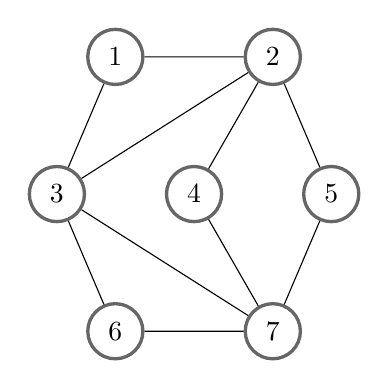
\begin{tikzpicture}[
roundnode/.style={circle, draw=black!60, fill=white!5, very thick, minimum size=7mm},
]
%Nodes
\node[roundnode](node4){4};
\node[roundnode](node3)[left=of node4] {3};
\node[roundnode](node5)[right=of node4] {5};
%lower level nodes 
\node[roundnode](node7)[below=of node4,xshift=10mm]  {7};
\node[roundnode](node6)[below=of node4,xshift=-10mm] {6};
%make the upper the nodes 
\node[roundnode](node1)[above=of node4,xshift=-10mm] {1};
\node[roundnode](node2)[above=of node4,xshift=10mm]  {2};
%Lines
\draw[-] (node2) -- (node4) -- (node7);
\draw[-] (node3) -- (node2) -- (node5);
\draw[-] (node3) -- (node7) -- (node5);
\draw[-] (node3) -- (node1) -- (node2);
\draw[-] (node3) -- (node6) -- (node7);
\end{tikzpicture}
\end{center}
Recall, that the definition of an independent set 
{\text {In a graph } G=(V, E), \text { we say a set of nodes }}{$S\subseteq V$ \text {is independent if no two nodes in } S \text { are joined by an edge.}} And we know it is to find a small independent set, a single node is simply an independent set. And in the graph above, we notice that {3,4,5} is an independent set and its size is 3, but can we get an independent bigger than 3, and indeed we can find a larger independent set with the set of nodes {1,4,5,6}. 

Note: No difference between an \textit{optimization version} of the problem: Find the largest independent set and the \textit{decision version} of problem : whether G has an independent set of size of at least some integer K. If we come up with algorithm to solve our \textit{optimization version}, then we automatically solve our \textit{decision version}. And this is a no brainer statement. Something less obvious but important, which if we solve \textit{decision version} for some integer k, then we can find a maximum independent set. In English, question like what is the size of the maximum independent set, you write an polynomial algorithm and you return 4 in our case. Another question: Is the size of the maximum size of independent 4? You would probably call the same algorithm or subroutine to solve this, an addition of checking (Boolean,it can be done in linear time), return true/false. All this is just to show the simple equivalence between decision and optimization. 

In the "Note", we specify the relationship with \textit{decision} and \textit{optimization}. Now we move on problem b). and smallest vertex cover problem, in English, means can you find the minimum number of vertex that can cover all the edges of a given graph. And as before, easy to find the largest one, which is including all the vertices, but hard in terms of finding the smallest one. 

Now, we know they are hard problem. But how do we show their relative difficulty? We need to show that Vertex Cover $\leq_{p}$ Independent Set and also Independent Set $\leq_{p}$ Vertex Cover. 

$//$ This can be seem as the f, the transformation between the two problems\\
To do this, we need a relationship between Independent Set and Vertex Cover. And the this relationship can be easily found in Our text book, But we need to prove it to agree with it. 
\begin{equation}
\begin{array}{l}{\text {Let } G=(V, E) \text { be a graph. Then } S \text { is an independent set if and only if}} \\ {\text {its complement } V-S \text { is a vertex cover. }}\end{array}
\end{equation}

\textbf{Proof.} Suppose that S is an independent set. Consider an edge $e=(u,v)$. Since S is independent, $u$ and $v$ can not both be in a S. So one of them must be in $V/S$. Following this idea we know that every single edge we are looking at, at least one end is in $V/S$, so $V/S$ is a vertex cover. 

Conversely, If $V/S$ is a vertex cover. Consider any nodes $u$ and $v$ in our $S$. If $u$ and $v$ is joined by edge $e$, then neither end of $e$ will fall into $V/S$, this contradict the assumption that $V/S$ is a vertex cover. So no two nodes in $S$ is joined by an edge, so $S$ is an independent set. 

$//$ The relationship here can be seem as an "h", show there is a
solution going both ways. \\
Therefore, our reduction is clear from (2): (we want to show the possibility of reducing the problem from either way)
\begin{enumerate}
    \item Independent Set \(\leq_{P}\) Vertex Cover.\\
    \textbf{Proof.} If we have a embedded PC to solve Vertex Cover, then we can decide whether G has an independent set of size at least $k$ by asking the the embedded PC whether G has a vertex cover of size at most $n − k$.
    \item Vertex Cover \(\leq_{P}\) Independent Set.\\
    \textbf{Proof.} If we have a embedded PC to solve Independent Set, then we can decide whether G has a vertex cover of size at most $l$ by asking the embedded PC whether G has an independent set of size at least $n − l$.
\end{enumerate}
From Homework 3, we do know that we have a polynomial time algorithm for Maximum Independent Set. So we see that there is an efficient algorithm for both of them. 

\section{Exact 4-SAT is NP-complete}
Recall From class the steps of proving a problem X is NP-complete.
\begin{enumerate}
    \item Prove X $\in$ NP;
    \item Pick an known NP-complete problem Y and show that it reduces to X; 
    \begin{enumerate}
        \item define f to convert instance of Y to instance of X;
        \item define h to convert X solution to Y solution; 
        \item solution to Y $\Rightarrow$ solution to X 
        \item solution to X $\Rightarrow$ solution to Y
        \end{enumerate}
\end{enumerate}

In class, we proved that a 3 SAT is NP-complete. Some people find it easy to see, but I don't think this is the case for me. So I will walk through it again. 

SATISFIABILITY(or SAT) is the problem of determining if there exists an interpretation that satisfies a given Boolean formula. In other word, it asks whether the variable of a given Boolean formula can be consistently replaced by the value TRUE or False in such a way that the formula evaluates to True. If this is the case, the formula is called satisfiable. 

SAT is NP-complete. Because Cook and Levin said so. 

Because our SAT is NP-complete, we can prove the completeness of 3 SAT. 
\begin{enumerate}
    \item 3SAT $\in$ NP, because to determine whether a boolean expression E in CNF is satisfiable, nondeterministically guess values for all the variables and then evaluate the expression. If E turns out to be true, then accept. This can be carried out in nondeterministic polynomial time. Thus 3SAT is in NP.
    \item We know that SAT is a NP-complete problem we need to show that it can be reduced to 3SAT, therefore Proving it is also NP-complete. 
    \begin{enumerate}
        \item A SAT instance has m clauses, consider an arbitrary clause. 
        $(a_1\vee a_2 \vee a_3 \vee ... \vee a_k)$
        \begin{enumerate}
            \item the function f converts this clause to 
            $$(a_1\vee a_2 \vee y_2)(\Bar{y_2}\vee a_3\vee y_3)...(\Bar{y_{k-3}} \vee a_{k-2} \vee y_{k-2})(\Bar{y_{k-2}}\vee a_{k-2} \vee a_k)$$
        \end{enumerate}
        \item The function h takes a 3SAT truth assignment and ignores the auxiliary variables. 
        \begin{enumerate}
            \item Suppose the SAT instance has a solution.Then our arbitrary clause must be satisfied, so some $a_i$ is True. 
            \begin{enumerate}[-]
                \item Consider $(\Bar{y_{i-2}}\vee a_i \vee y_i)$
                So, let's set $Y_{i-1}$ = T, $y_i$ = F, look at the CNF above and setting auxiliary variable to the left half as true and set the right half as false, and keep doing this we will have a 3SAT solution. 
            \end{enumerate}
            \item Suppose 3SAT instance has a solution, Claim $a_i$ = T for some i. Suppose not: all $a_i=F$, then 3SAT clause means only $y_i$ matters and this is not satisfiable. So $a_i=T$ for some i so there is a solution for SAT. 
        \end{enumerate}
    \end{enumerate}
\end{enumerate}

After showing the steps and the idea presented in class, now we know that 3SAT is NP-complete. So now we can move on prove that EXACT 4 SAT is NP-complete using the same idea. 

\begin{enumerate}
    \item First, 4-SAT is in NP, we can write a non-deterministic polynomial-time algorithm which takes a 4-SAT instance and a proposed truth assignment as
input. This algorithm evaluates the 4-SAT instance with the truth assignment. If the 4-SAT instance evaluates to true, the algorithm outputs yes;
otherwise, the algorithm outputs no. This runs in polynomial time.
\item We know that 3SAT is a NP-complete problem we need to show that it can be reduced to EXACT 4SAT, therefore Proving it is also NP-complete. 
\begin{enumerate}
    \item A 3SAT Instance has m clause, consider an arbitrary clause $(a_1 \vee a_2 \vee a_3)$
    \begin{enumerate}
        \item the function f convert this clause to 
        $$(a_1 \vee a_2 \vee a_3 \vee y) \wedge(a_1 \vee a_2 \vee a_3 \vee \Bar{y})$$
        and y is the auxiliary variable. 
    \end{enumerate}
    \item The function h takes a 4SAT truth assignment and ignores the auxiliary variables.
    \begin{enumerate}
        \item Suppose 3SAT instance has a solution.Then our arbitrary clause must be satisfied, so some literal is True. Then we have a solution for our 4SAT since $a_1$ or $a_2$ or $a_3$ is true and connected by "OR" so the auxiliary is irrelevant in this case. 
        \item Suppose 4SAT instance has a solution. Claim some literals is True. Suppose not. All literal is false.Then we only care about our auxiliary and it will not be satisfiable, because y $\wedge$ $\Bar{y}$ returns False no matter what. So it is not satisfiable. So some literals equal to T, so there is a solution to 3SAT.
        \end{enumerate}
\end{enumerate}
\end{enumerate}
In conclusion, EXACT 4 SAT is NP-complete.
\newpage
\section{Graph Coloring and Course Scheduling}
We know K-coloring is NP-complete from the question. So the questions :given a fixed number of time slot, and the time slot can be seem as our "k".\\
\begin{center}
%this is figure 1 
\begin{minipage}[b]{.3\linewidth}
\begin{tikzpicture}[
roundnode/.style={circle, draw=black!60, fill=white!5, very thick, minimum size=7mm},
]
%Nodes
\node[roundnode](nodeT){T};
\node[roundnode](nodeF)[left=of nodeT] {F};
%make the upper the nodes 
\node[roundnode](nodeBase)[above=of node4,xshift=-10mm] {B};
%Lines
\draw[-] (nodeT) -- (nodeF) -- (nodeBase)--(nodeT);
\end{tikzpicture}
\captionof{figure}{3-coloring(example)}
\end{minipage}
%Figure 2 
\begin{minipage}[b]{.3\linewidth}
\begin{tikzpicture}[
roundnode/.style={circle, draw=black!60, fill=white!5, very thick, minimum size=7mm},
]
%Nodes
\node[roundnode](nodeT){$Class$};
\node[roundnode](nodeF)[left=of nodeT] {$\Bar{Class}$};
%make the upper the nodes 
\node[roundnode](nodeBase)[above=of node4,xshift=-10mm] {B};
%Lines
\draw[-] (nodeT) -- (nodeF) -- (nodeBase)--(nodeT);
\end{tikzpicture}
\captionof{figure}{course schedule graph}
\end{minipage}
    
\end{center}



\begin{enumerate}
    \item We can easily see that Course Scheduling is a NP problem. Because we are simply assigning proposed truth assignment and see if there is a conflict or not and eventually see if it is right or wrong. So this can be run in polynomial time. 
    \item We know from the problem that k-coloring is a NP-complete problem, we will prove it by reducing k-coloring problem to  the course scheduling problem.
    \begin{enumerate}
        \item The "f" from my understanding by talking more in-depth with professor Ballard, well from my perspective, probably not so for him, is converting our know problem,k-coloring,to something resemble our asked problem,course scheduling. In this case I think it is pretty obvious. We can imagine a graph where the vertex is the classes with conflicts and they are connected by the edges. And in order to avoid a time conflict we need to assign different colors, or time slot, to the classes. And no two classes can have the same time slot, meaning, two vertex connect by the same edge can not have the same color.
        \item Now,we need to find the "h". 
        \begin{enumerate}
            \item Suppose that we that have a solution for our K-coloring instance, meaning that no vertex of the same edge share the same color. Then we will also have a solution to the course scheduling instance, since no two conflict connecting the same classes will have the the same time slot(color). 
            \item The same argument also goes from course scheduling to k-coloring. No two two conflicted class have the same time slot$\rightarrow$ No two vertices connected by the same edge have the same color. 
        \end{enumerate}
    \end{enumerate}
\end{enumerate}
In conclusion, course scheduling is NP-complete. 

\end{document}; 